%%%%%%%%%%
% [TODO] %
%%%%%%%%%%
% [ ] Mini-intro
% [ ] Anatomy of ASR system
% [ ] Parlato-hmm
% [ ] surfphono
% --- [ ] Check if batch is bigram or trigram
% --- [ ] Explain ABC methodology
% [ ] Mini-discussion

%%%%%%%%%%%%%%%%%%%%%%
% Chapter mini-intro %
%%%%%%%%%%%%%%%%%%%%%%

%%% Short BG
%\subsection{ASR tools as models of perception}


%%% Research question + alternatives


%%% Plan


%%%%%%%%%%%%%%%%%%%
% General methods % %
%%%%%%%%%%%%%%%%%%%

\section{Anatomy of an HMM-based speech recogniser}
In this chapter we used Hidden Markov Model (HMM)-based speech recognisers as model of human perception.

{\color{red}
...
[Here equation + graph of modules]
}


In the field of ASR, Neural Network (NN)-based speech recognisers are king. In spite of better performance of NN-based ASR systems, we decided to use more well-understood HMM-based recognisers. Indeed, before the decoding step, these models offer a clear separation between the acoustic model (AM; i.e., mapping between phoneme categories and acoustics) and the language model (LM; i.e., frequencies of word/phoneme sequences). This allowed us to test ASR systems with different LMs while keeping the AM constant, as well as adapting LMs to mimic the experimental paradigms used when testing human participants.
We will now present the components of an HMM-based ASR system in more detail.

\subsection{Corpora}

In order to train and test our ASR system, we needed transcribed speech corpora. These corpora consisted of speech recordings which have been annotated; for each utterance, we have a more or less detailed transcription of what was said.
While the ideal annotation is the one for which phoneticians have provided phoneme categories, as well as their boundaries, often we might only have access to by-utterance annotations where we are only provided with a sequence of words/phonemes for each utterance. In these cases, we rely on forced alignment to automatically find phoneme boundaries.

In the following sections we have trained ASR systems with different ``native'' languages, namely Japanese (JP) and Korean (KR). These languages were of particular interest because of their relatively restrictive phonotactic constraints with regards to consonant clusters, as well as the availability of spontaneous speech corpora, which we will now present. 

\paragraph{Corpus of Spontaneous Japanese (CSJ)}
As the name suggests, the CSJ \cite{maekawa2003} contains recordings of spontaneous Standard Japanese. The corpus is composed of two subparts: (1) academic presentation speech (APS), which consists of live recordings of academic presentations, and (2) simulated public speech (SPS), where speakers presented everyday topics in front of a small audience. For our models we only kept SPS, which is more representative of everyday conversations at the level of the lexicon, and has a more balanced population than the young male-dominated APS.
Our subset of the corpus contained 400,547 utterances produced by 594 speakers (331 female, 263 male), with an average of 674.3 utterances per speaker.  
Recordings were manually transcribed by native speakers of Japanese. Phoneme boundaries were {\color{red}manually adjusted, however this alignment was not used when our models, as it was overwritten by forced alignment}.

\begin{itemize}
\item Train-test division (n utterances, time)
\item ...
\end{itemize}

\paragraph{Korean Corpus of Spontaneous Speech (KCSS)}

The KCSS \cite{yun2015} consists of recordings of spontaneous Seoul Korean. Forty speakers aged 10 to 49 (5 female speakers and 5 male speakers per decade) were recorded in a quiet room, for approximately 1 hour each. Speech was ellicited through questions related to the speakers' personal opinions, habits, acquaintances, etc.      
Recordings were manually transcribed by native speakers of Korean. We used phonetic transcriptions faithful to actual pronunciations which, for instance, include phonetic reduction (e.g., \textit{yesterday} transcribed as \textipa{/jESeI/} instead of the canonical \textipa{/jEst\textrhookschwa deI/}). Transcriptions include {\color{red}manually adjusted} phoneme boundaries, as well as word syllabification.
The corpus contains 126,132 utterances produced by 40 speakers (as explained above), with an average of 3153.3 utterances per speaker. 

\begin{itemize}
\item Train-test division (n utterances, time)
\item ...
\end{itemize}

\subsection{Features}
\begin{itemize}
\item What are MFCCs
\item CMVN
\item Pitch
\item ...
\end{itemize}

\subsection{Acoustic model}
\begin{itemize}
\item Monophone model - also, why?
\item Number of gaussians
\item Number of states
\item Duration included in state transitions 
\item ...
\end{itemize}
    
\subsection{Language models}
\begin{itemize}
\item WFSTs
\item Words \& phones 
\item n-grams
\item ...
\end{itemize}

\subsection{Decoding}
\begin{itemize}
\item Lattice generation
\item Acoustic and LM scores 
\item nbest
\item CTM
\item ...
\end{itemize}

\subsection{Scoring: Assessing native performance}
\begin{itemize}
\item Lexicon-based decoding
\item Phonetic-based decoding
\end{itemize}

%%%%%%%%%%%%
% Parlato2 %
%%%%%%%%%%%%
\newpage
\section{{\color{red}Parlato-hmm}} \label{3-parlato-hmm}
\subsection{Introduction}
\subsection{Methods}
\subsubsection{Stimuli}
We used the same stimuli as in sections \ref{2-parlato} and \ref{2-parlato-dur}. As a reminder, a native French speaker recorded 54 items with the structure $V_{1}C_{1}C_{2}V_{2}$, with $V_{1}$ and $V_{2}$ vowels from the set \{/a/, /i/, /u/\}, and $C_{1}C_{2}$ a cluster from the set \{/bg/, /bn/, /db/, /dg/, /gb/, /gn/\} (e.g. /abgi/).

\subsubsection{Language models}
In order for the decoding task to be analogous to the experiment described in sections \ref{2-parlato_per} and \ref{2-parlato-dur}, trial-specific language models were constructed, as shown in Figure \ref{fig:parlato_G}. Thus, when decoding a $V_{1}C_{1}C_{2}V_{2}$ stimulus, the perception model was only given the possibility to transcribe it as $V_{1}C_{1}(V_{3})(SIL)C_{2}V_{2}$, where phones between parentheses are optional and $V_{3}$ was from the set of vowels \textipa{/a, e, i, o, u/}. In this section our language model was only used to constrain the list of possible outputs from decoding; one output was not more probable than another based on the language models alone. Therefore, here we used a null language model (\textsc{0P-LM}), meaning that the quality of the epenthesized vowels was only be determined by the acoustic match.

\begin{figure}[htb]
\centering
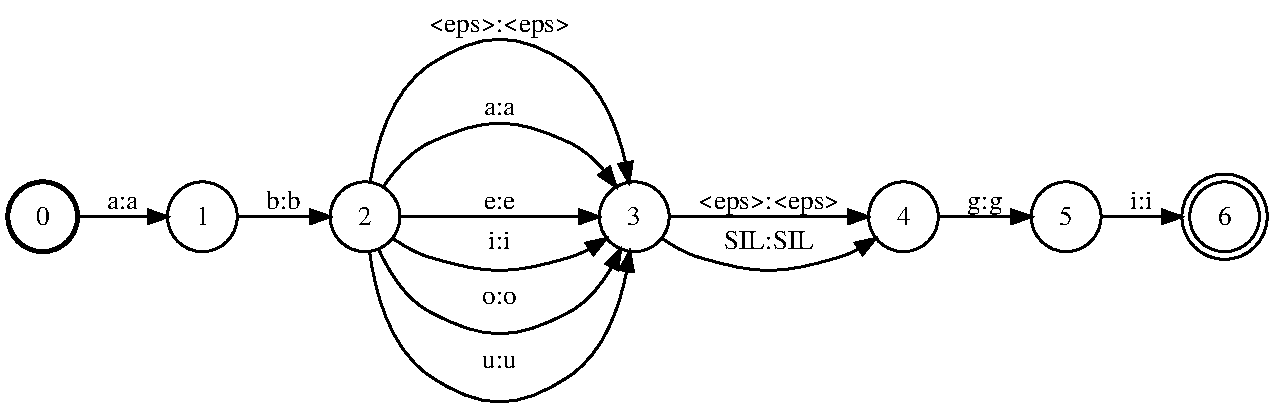
\includegraphics[width=0.8\linewidth]{chapter03/parlato_hmm_Gfst.pdf}
\caption{Constrained language model used for decoding the stimulus \textipa{/abgi/}. Nodes in the graph represent states, edges represent transitions between states (here: phonemes). The lack of weights on edges issued from a same node (e.g., between states 2 and 3) indicates that path selection is entirely decided by acoustic scores when decoding experimental items, with an acoustic scale of $0.1$. An optional silence can be inserted by the model between states 3 and 4.}
\label{fig:parlato_G}
\end{figure}

\subsubsection{Identification task simulation}
After decoding the stimuli, we obtained for each possible transcription of each item the corresponding acoustic and language model scores. From these we derived the item posteriorgrams, which indicate how probable a given transcription was given the audio input. We used these probabilities as proxies of the probability that a listener might exploit when performing reverse inference during speech perception, and therefore, the probabilities used when responding in an identification task. 

As such, for each item, we obtained a six-dimensional vector $ident_{model} = [p_{none}, p_{a}, p_{e}, p_{i}, p_{o}, p_{u}]$, containing a discrete probability distribution, with a probability mass function linking the identification task options 'none', 'a', 'e', 'i', 'o', 'u', to their respective probabilities (i.e., posteriorgrams).
We can define the human equivalent $ident_{human} = [p_{none}, p_{a}, p_{e}, p_{i}, p_{o}, p_{u}]$, which contains the percentage of responses for each item, after aggregating all participant responses. 

\subsubsection{Data analysis}
Statistical analyses were performed with the R statistical software \cite{R-base}, using Markov chain Monte Carlo generalised linear mixed-models \cite{R-MCMCglmm, R-coda}. These Bayesian models sample coefficients from the posterior probability distribution conditioned on the data and given priors. We used priors that are standard for linear models. Model convergence was assessed by visual inspection of trace plots and the Gelman–Rubin convergence diagnostic \cite{gelman1992}, using eight chains with different initialisations. Effects were considered statistically significant if the 95\% highest posterior density (HPD) interval estimated for the coefficient of interest did not include zero. We report both the posterior mode and the 95\% HPD interval.  

In order to assess the influence of $V_{1}$ and $V_{2}$ (henceforth: flanking vowels) on epenthetic vowel quality (/i/ or /u/), we chose as fixed effect for our statistical models \textsc{Number of Same Flanking Vowels} (\textsc{NSFV}; considered as a continuous variable with values 0, 1, or 2 instead of a factor with 3 levels, in order to reduce the number of model parameters and promote convergence). Due to the almost null variance and the consequent poor trace plot for the random intercept \textsc{Cluster}, we did not include it in the statistical models. Our response variable was the continuous variable \textsc{Posteriorgram}.\footnote{Responses by human participants and exemplar models were given by trial; therefore in previous cases the response variable was binomial.}

\subsection{Results}
\subsubsection{Overall similarity}
\begin{figure}[H]
  \centering
  \begin{overpic}[page=1, width=0.5\linewidth]{chapter03/parl_hmm_figs}\end{overpic}
  \caption{\textit{Distribution of posteriorgrams obtained when decoding with a ``null'' language model (0P-LM). The box and whiskers plots display the distribution of posteriorgrams across experimental items.}}
  \label{fig:parl_hmm_overall}
\end{figure}
Figure \ref{fig:parl_hmm_overall} shows the distribution of posteriorgrams for each response, with one datapoint per stimulus. The most probable transcriptions for the stimuli were ``none'' (26.7\%), ``u'' (24.3\%) and ``i'' (22.5\%).  While these were also the most frequent responses given by human participants (``none'': 13.1\%; ``u'': 63.1\%; ``i'': 15.3\%), the preponderance of \textipa{/u/}-epenthesis is missing in the model.

% > agr.ep (model average pgram)
%   resp          x
% 1 none 0.26667043
% 2    a 0.04802057
% 3    e 0.12948173
% 4    i 0.22494707
% 5    o 0.08715853
% 6    u 0.24372167

% > colMeans(d.comp.per[-1]) (human average resp)
%     p.none        p.a        p.e        p.i        p.o        p.u 
% 0.13071895 0.01416122 0.02505447 0.15250545 0.04684096 0.63071895 

In order to have a general idea of the model's ability to reproduce human behaviour, we computed the distance between human and model response patterns by computing the normalized Euclidean distance between $ident_{model}$ and $ident_{human}$, within each experimental item. The mean (and median) distance was $0.44$. This is higher than what was obtained by the best exemplar model in section \ref{2-parlato-dur} (mean distance: $0.33$; median distance: $0.21$); however remember that exemplar models were only able to output ``i'', ``o'', and ``u'' as responses. When computing the distance by taking into account the missing responses ``none'', ``a'', and ``e'', responses from the best JP exemplar model have a mean distance of $0.39$ (median: $0.30$) with respect to human responses.

While it might be tempting to conclude that the exemplar model was superior compared to the HMM model, it is important to note that the task modelled by the HMM-based model is closer to the task participants were subjected to (6-alternative forced choice identification task) than the exemplar models (3-AFC identification task). Technically, a ``dummy'' model in the 3-AFC situation, where all options are equally probable, would output ``u'' for $33\%$ of the trials. This is a higher percentage of \textipa{/u/}-epenthesis than the $24.3\%$ from our current model. Since ``u'' is by far the most frequent response given by human participants (and ``a'' and ``e'' are very infrequent), even a dummy 3-AFC \textipa{\{``i'', ``o'', ``u''\}} model might outclass our 6-AFC \textipa{\{``none'', ``a'', ``e'', ``i'', ``o'', ``u''\}} ASR system.

As such, we believe that it is unfair to compare Euclidean distances between models based on different tasks. We can, however, see if the ASR-based model reproduces the qualitative effects that the best exemplar model was able to mimic.

\subsubsection{Effect of coarticulation}

\paragraph{/i/-epenthesis}

The left panel of Figure \ref{fig:parl_hmm_iu} shows the posteriorgrams for \textipa{/i/}-epenthesis given by our ASR-based model with a ``null'' language model (\textsc{0P-LM}).
The main effect of \textsc{NSFV} was significant (mode: $0.10$, HPD: $[0.01, 0.18]$). An increased number of \textipa{/i/} flanking vowels resulted in higher posteriorgrams for stimuli transcriptions with \textipa{/i/} epenthesis.

\begin{figure}[H]
  \centering
  \begin{overpic}[page=2, width=0.4\linewidth]{chapter03/parl_hmm_figs}\end{overpic}
  \hspace{1cm}
  \begin{overpic}[page=3, width=0.4\linewidth]{chapter03/parl_hmm_figs}\end{overpic}
  \caption{\textit{Posteriorgrams for \textipa{/i/}-epenthesis (left) and \textipa{/u/}-epenthesis (right) obtained when decoding with a ``null'' language model (0P-LM). The box and whiskers plots display the distribution of posteriorgrams across experimental items, represented by individual dots.}}
  \label{fig:parl_hmm_iu}
\end{figure}

\paragraph{/u/-epenthesis}
The right panel of Figure \ref{fig:parl_hmm_iu} shows the posteriorgrams for \textipa{/u/}-epenthesis given by our ASR-based model with a ``null'' language model (\textsc{0P-LM}).
The main effect of \textsc{NSFV} was not significant (mode: $0.04$, HPD: $[-0.02, 0.10]$). Therefore, an increased number of \textipa{/u/} flanking vowels did not result in significantly higher posteriorgrams for stimuli transcriptions with \textipa{/u/} epenthesis.

\subsection{Discussion}
%%% Summary

%%% Duration in ASR?

%%%%%%%%%%%%%%%%%%%%%%%%%%
% m-/ahpa/ + parlato_lms %
%%%%%%%%%%%%%%%%%%%%%%%%%%
\newpage
\section{{\color{red}Investigating surface phonotactics}} \label{3-surfphono}

\small{\textit{{\color{red}ADD ACKNOWLEDGEMENTS THOMAS + EMMANUEL.\\}}}

\subsection{Introduction}
\subsection{Experiment 1: {\color{red}Parlato-lms}}
\subsubsection{Methods}
\paragraph{Stimuli}
We used the same stimuli as in sections \ref{2-parlato}, \ref{2-parlato-dur}, and \ref{3-parlato-hmm}. As a reminder, a native French speaker recorded 54 items with the structure $V_{1}C_{1}C_{2}V_{2}$, with $V_{1}$ and $V_{2}$ vowels from the set \{/a/, /i/, /u/\}, and $C_{1}C_{2}$ a cluster from the set \{/bg/, /bn/, /db/, /dg/, /gb/, /gn/\} (e.g. /abgi/).

\paragraph{Language models}
In this section, we investigate the type of phonotactic information used by Japanese listeners when perceiving foreign speech that does not conform to native phonotactics. We test 5 types of language models (LM) when decoding our $V_{1}C_{1}C_{2}V_{2}$ items; these differ only in the weights given to edges between nodes 2 and 3 in the graph shown in Figure \ref{fig:parlato_G}: 
\begin{enumerate}
    \item A null language model (\textsc{0P-LM}), which implies that listeners base their decoding of consonant clusters on phonetics alone, without using information on phonotactics (as in section \ref{3-parlato-hmm}).
    \item A phone-unigram language model (\textsc{1P-LM}), which implies that listeners do not take neighbouring phonemes into consideration when decoding the consonant clusters; only the frequency of the vowel $V_{ep}$ to be epenthesized (compared to that of $C_{2}$) is taken into account when choosing epenthetic vowel quality.
    \item An online phone-bigram language model (\textsc{2PO-LM}), which implies that listeners decode the clusters as they hear them (decoding is done from the start of the item). Here the choice of epenthetic vowel is modulated by $C_{1}V_{ep}$ and $C_{1}C_{2}$ diphone frequencies. 
    \item A retro phone-bigram language model (\textsc{2PR-LM}), which implies that listeners decode the clusters based on the most recent information (decoding is done from the end of the item). Here the choice of epenthetic vowel is modulated by $V_{ep}C_{2}$ and $C_{1}C_{2}$ diphone frequencies.
    \item A batch phone-bigram language model (\textsc{2PB-LM}), which implies that listeners decode the item considering the entire structure, with bigrams. Here the choice of epenthetic vowel is modulated by $C_{1}V_{ep}$ and $V_{ep}C_{2}$ (and $C_{1}C_{2}$) diphone frequencies.  
\end{enumerate}


\paragraph{Identification task simulation}
We used the same procedure as in section \ref{3-parlato-hmm}.

\paragraph{Data analysis: ABC easy as 123}
% Reasoning
% Model selection
% Parameter tuning

{\color{red}Here: explain ABC}

In order to select the language model which best predicted our behavioural data, we inferred the \textit{a posteriori} distributions of the weights given to acoustic model and language model in {\color{red}equation \ref{}}, using ABC. The following aggregated data were used as summary statistics:

\begin{itemize}
\item \textsc{\%none}: Proportion of ``none'' responses (no epenthesis)
\item \textsc{\%$V_{1}\underline{\vee}V_{2}$}: Proportion of trials where the epenthesized vowel shares the quality of either $V_{1}$ or $V_{2}$, with $V_{1} \neq V_{2}$
\item \textsc{\%$V_{1}\land V_{2}$}: Proportion of trials where the epenthesized vowel shares the quality of both $V_{1}$ and $V_{2}$, with $V_{1} = V_{2}$
\item \textsc{\%default}: Proportion of default \textipa{/u/}-epenthesis over all trials
\item \textsc{\%coronal}: Proportion of \textipa{/o/}-epenthesis following coronal consonants over all trials with clusters containing coronal consonants 
\end{itemize} 

\subsubsection{Results and Discussion}
\subsection{Experiment 2: {\color{red}m-/ahpa/}}
\subsubsection{Methods}
\paragraph{Stimuli}
We used the same stimuli as in section \ref{2-ahpa}. As a reminder, we recorded 3 speakers producing disyllabic $V_{1}C_{1}C_{2}V_{1}$ and trisyllabic $V_{1}C_{1}V_{2}C_{2}V_{1}$, with $V_{1}$ a flanking vowel in the set \textipa{/a, e, i, o, u/}, $C_{1}$ \textipa{/h/} or /k/, and $C_{2}$ a fixed consonant, /p/ (e.g, \textipa{/ahpa/}, \textipa{/ahapa/}). By splicing the disyllabic natural control items (e.g., \textipa{/ahpa/}), we obtained disyllabic spliced control items (e.g., \texorpdfstring{\textipa{/ah\textsubscript{a}pa/}}{}), disyllabic spliced test stimuli (e.g., \texorpdfstring{\textipa{/ah\textsubscript{u}pa/}}{}), and trisyllabic spliced fillers (e.g., {\textipa{/ahapa/}). Therefore, within each speaker, all stimuli of the same structure (in our example, \textipa{/ah($V$)pa/} items) are acoustically identical on their flanking vowels.
  
\paragraph{Language models}
We used the same language models as in Experiment 1, adapted to the $V_{1}C_{1}C_{2}V_{1}$ items used in this experiment. A graphical representation can be found in Figure \ref{fig:m-ahpa_G}.
  
\begin{figure}[htb]
    \centering
    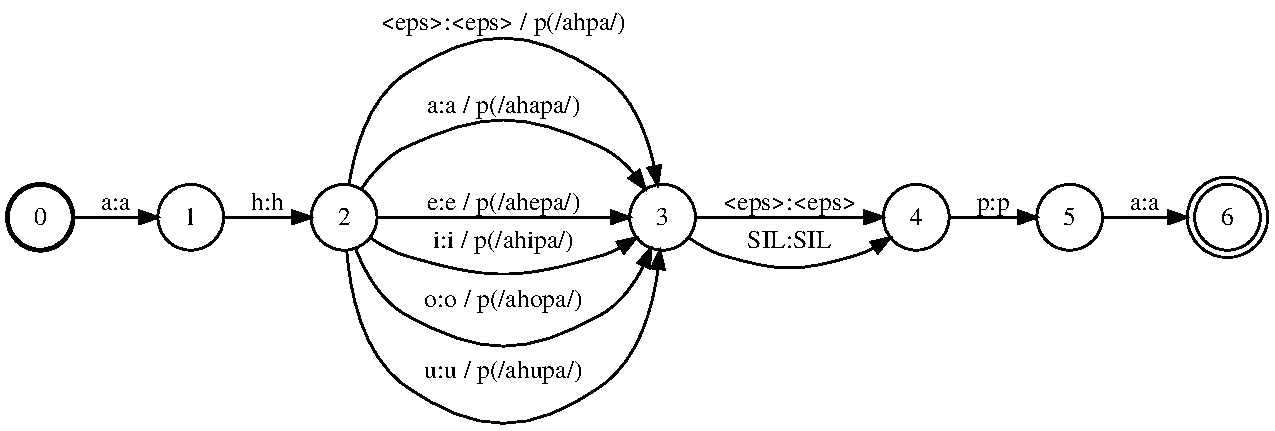
\includegraphics[width=0.8\linewidth]{chapter03/m-ahpa_Gfst.pdf}
    \caption{Constrained language model used to test the models (here: LM for \textipa{/ahpa/} trials). Nodes in the graph represent states, weighted edges represent transitions between states (here: phonemes). When relevant, weighted edges are labeled with the probability to choose that edge when decoding, which affects the final language model score of each possible path. These scores are then combined with acoustic scores when decoding experimental items.}
    \label{fig:m-ahpa_G}
\end{figure}
  
\paragraph{Identification task simulation}
We used the same procedure as in section \ref{3-parlato-hmm}.

\paragraph{{\color{red}Data analysis}}
% Refer to previous experiment
% Model selection
% Parameter tuning

In order to select the language model which best predicted our behavioural data, we inferred the \textit{a posteriori} distributions of the weights given to acoustic model and language model in {\color{red}equation \ref{}}, using ABC. The following aggregated data were used as summary statistics:

\begin{itemize}
\item \textsc{\%none}: Proportion of ``none'' responses (no epenthesis)
\item \textsc{\%coart}: Proportion of trials where the epenthesized vowel shares the quality of the coarticulation within the consonant (including \textipa{/u/} coarticulation).
\item \textsc{\%default}: Proportion of default \textipa{/u/}-epenthesis over all trials
\end{itemize}

Since we saw in section \ref{2-ahpa} that patterns of epenthesis differed depending on whether the consonant cluster was \textipa{/hp/} or \textipa{/kp/}, we computed these summary statistics twice, one set per consonant cluster. As such, the final number of statistics was six. 

\subsubsection{Results and Discussion}
\subsection{Discussion}

%%%%%%%%%%%%
% k-epenth %
%%%%%%%%%%%%
\newpage
\section{{\color{red}Do we need to go deeper? Are surface phonotactics enough?}} \label{3-k-epenth}
\subsection{Introduction}
\subsection{Methods}
\subsubsection{Stimuli}
\paragraph{Identification task simulation}
\subsubsection{Data analysis}
\subsection{Results}
\subsection{Discussion}
%%%%%%%%%%%%%%%%%%%%%%%%%%%
% Chapter mini-discussion %
%%%%%%%%%%%%%%%%%%%%%%%%%%%
\section{Conclusions}
%%% Summary

%%% Short discussion

%%% Limitations

%%% Conclusions